\section{Bernie Stone Case Study}\label{sec:case_study}
This section discusses the case of Bernie Stone, which is the leading motivating evidence of this behavior for this setting.
Bernie Stone was an alderman in Chicago's 50th ward from 1973 to 2011.
He was well known for his, ``political philosophy.''

\begin{quotation}
    ``You take care of the people who take care of you — you know, the people who voted for you, That’s not Chicago politics, that’s Politics 101.'' - Alderman Bernie Stone (50th ward) \citep{BGA_berniequote}
\end{quotation}

In fact an alderman who grew up in the 50th ward once remarked that,

\begin{quotation}
    ``Well, I grew up in the 50th Ward and you know, God bless [the late former Ald.] Bernie Stone, may he rest in peace, but I remember crossing California going west, every street was resurfaced almost every year. They always had brand new lighting and then east of California, where he would lose the precincts consistently, I mean the streets were in shambles. Many people felt he was spending the bulk of the menu money west of California, where he was getting the bulk of the vote.'' - Alderman Carlos Ramirez-Rosa (35th Ward) \citep{ramirezrosaquote}
\end{quotation}

This quote is a clear example of the type of behavior that this paper seeks to investigate.
This phenomenon could not be quantified previously because the CDOT did not make the 2005-2011 documents publicly available. 
Furthermore, the 2011-2022 data was in PDF form, making locating the spending tedious and difficult.
This paper is the first to put numbers to this anecdotal evidence.
Figure~\ref{fig:stone_support_maps} depicts the precincts that supported Stone in the 2007 runoff election and the precincts that gave Stone the most individual contributions.
Combined, both maps show that the southwestern portion of the ward is the most supportive of Stone, on average.
The two are also somewhat correlated, with a correlation coefficient of 0.14.
\begin{figure}[H]
    \centering
    % First subfigure
    \begin{subfigure}[b]{0.45\textwidth} % [b] aligns at the bottom
    \includegraphics[width=\textwidth]{input/contribution_map_stone_ward_50_2003_2011.png}
    \caption{Campaign contributions to Alderman Stone, 2003-2011}
    \end{subfigure}
    \hfill % This adds some space between the two subfigures
    % Second subfigure
    \begin{subfigure}[b]{0.45\textwidth}
    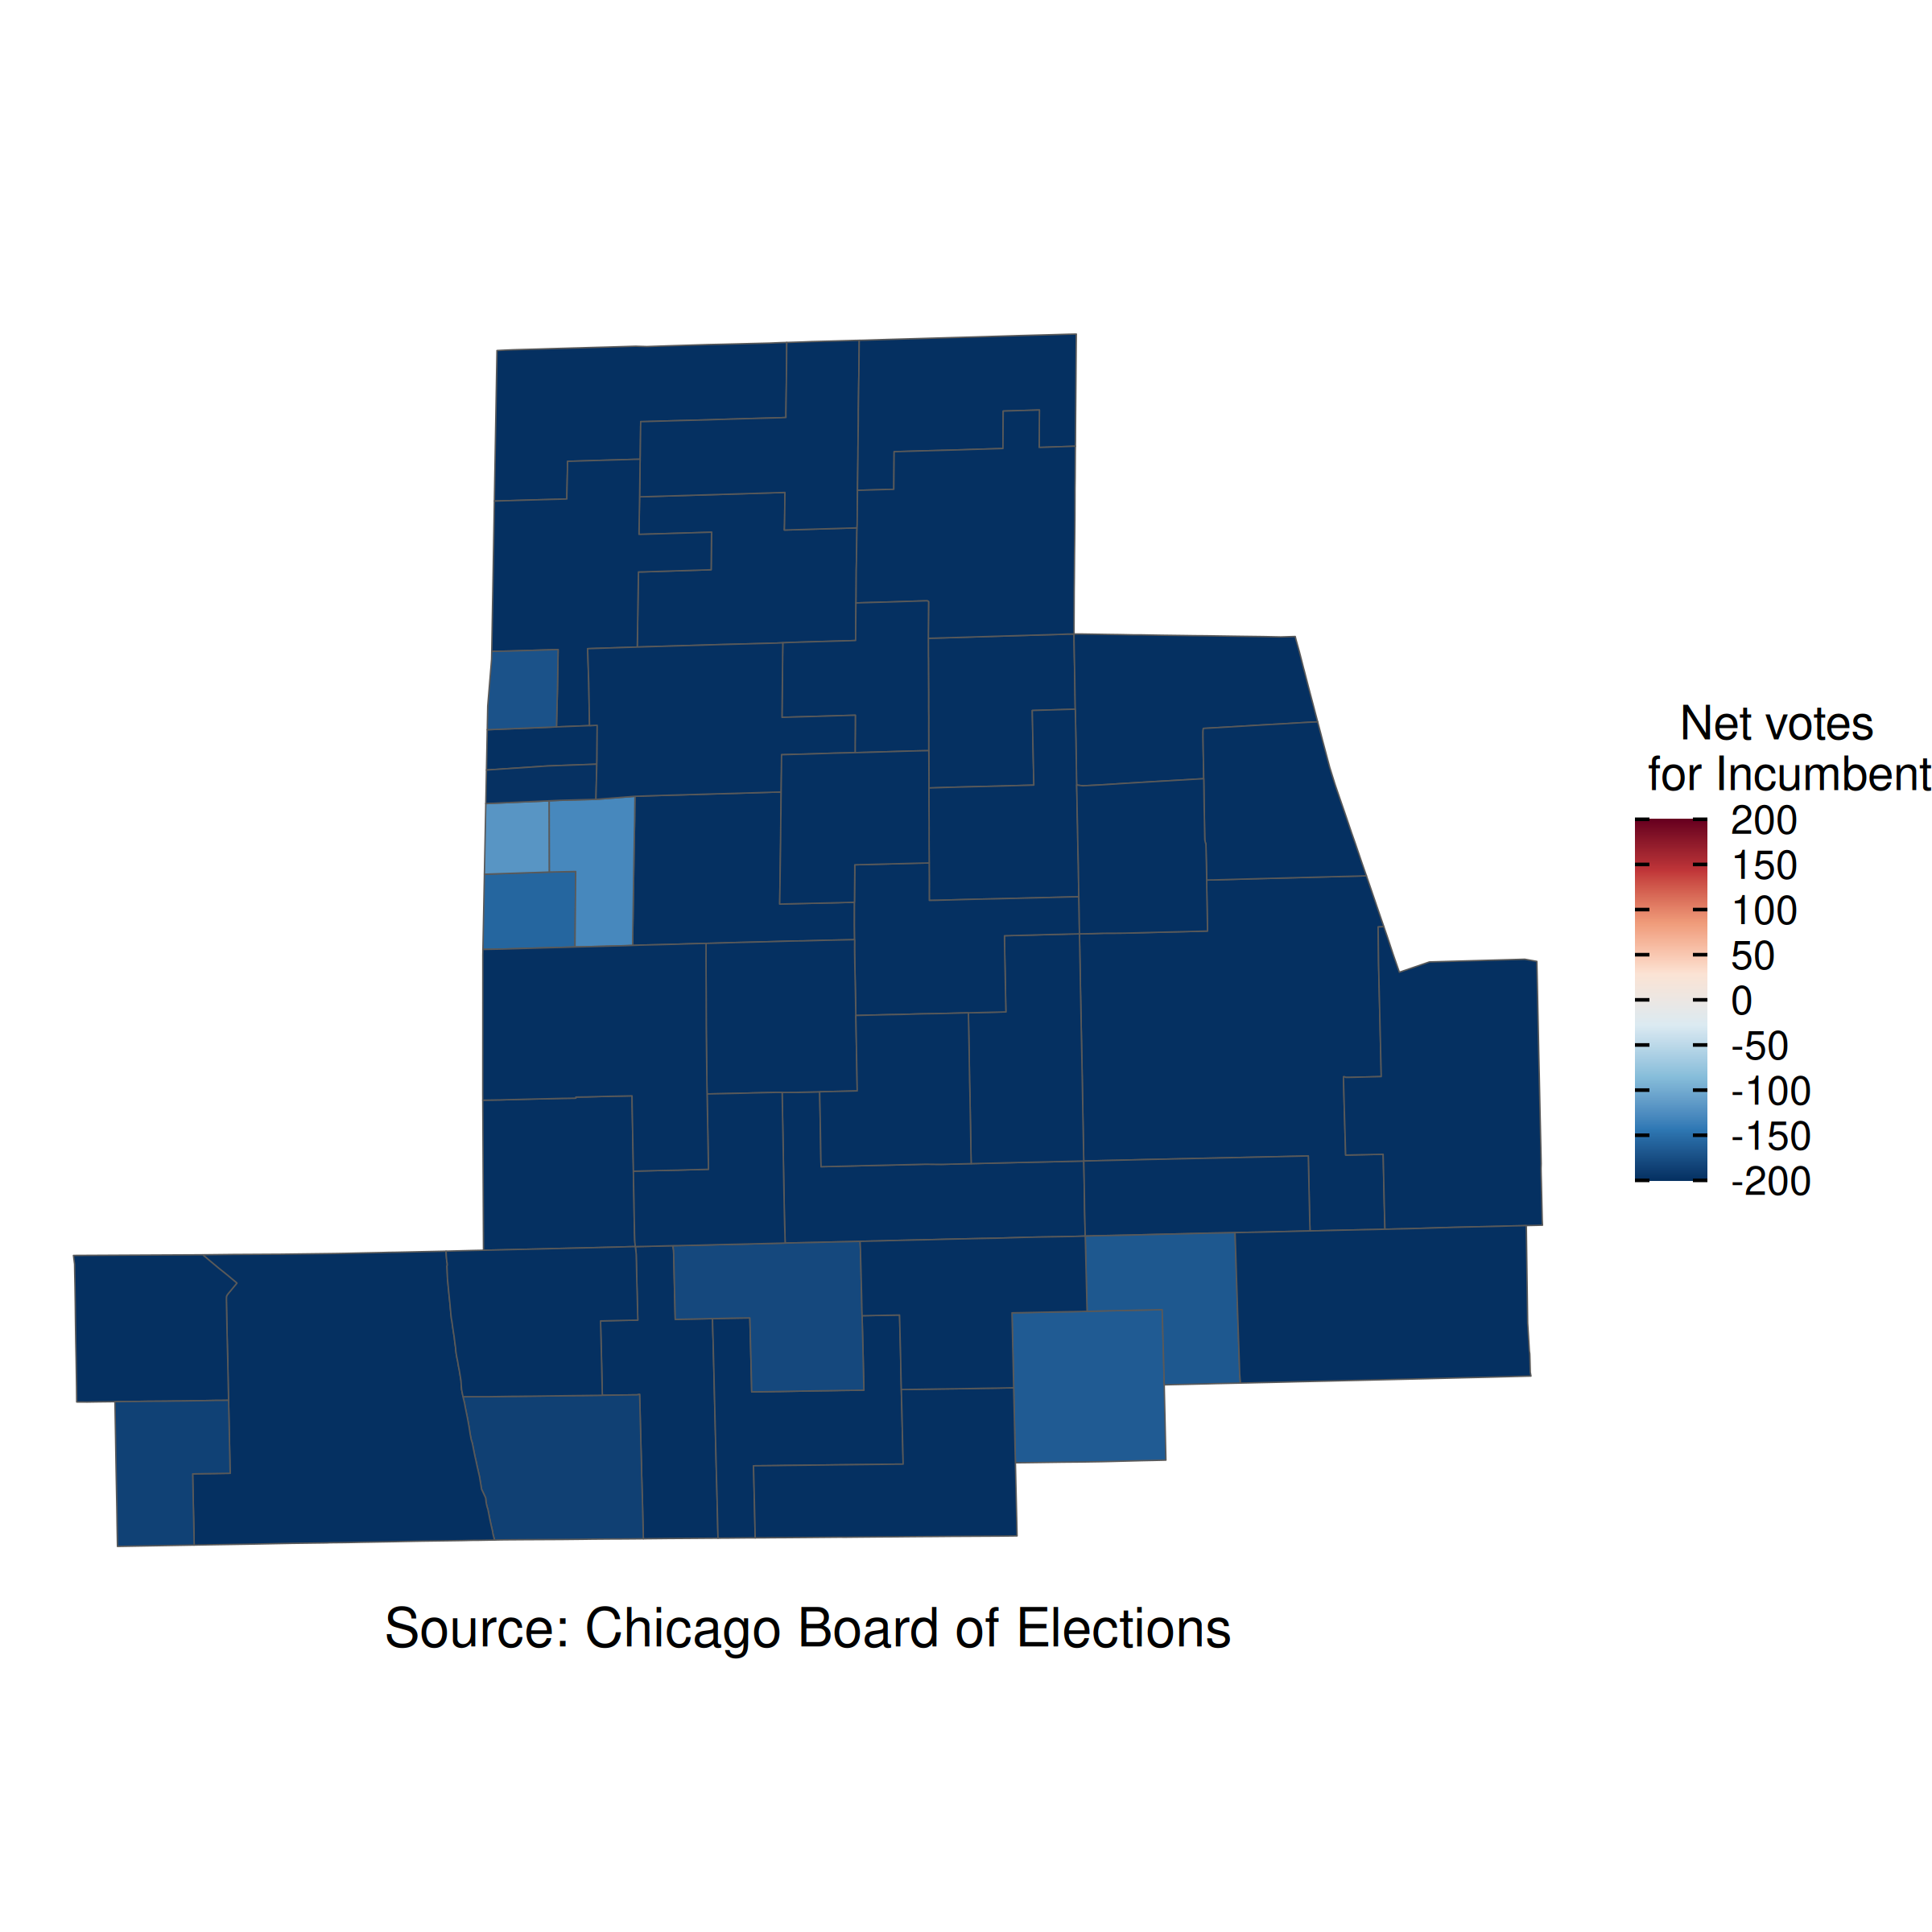
\includegraphics[width=\textwidth]{input/ward_50_2007_runoff_incumbent_precinct_results.png}
    \caption{Net votes for Alderman Stone, 2007}
    \end{subfigure}
    \caption{Alderman Stone's support in the 50th ward}
    \label{fig:stone_support_maps}
\end{figure}

Figure~\ref{fig:stone_spending_timeline} gathers the top and bottom quintile of 44 precincts in the 50th ward by contributions to Stone and shows the average fraction of the total located menu budget spent in each quintile and the rest of the ward.
Note that the precincts that contributed the most to Stone's campaign are the same precincts that contributed the most net votes to Stone in the 2007 runoff election.
After his reelection in 2007, Stone's spending per precinct was heavily concentrated in the precincts that supported him.
After his defeat, spending per precinct is much more evenly distributed across the ward.

\begin{figure}[H]
    \centering
    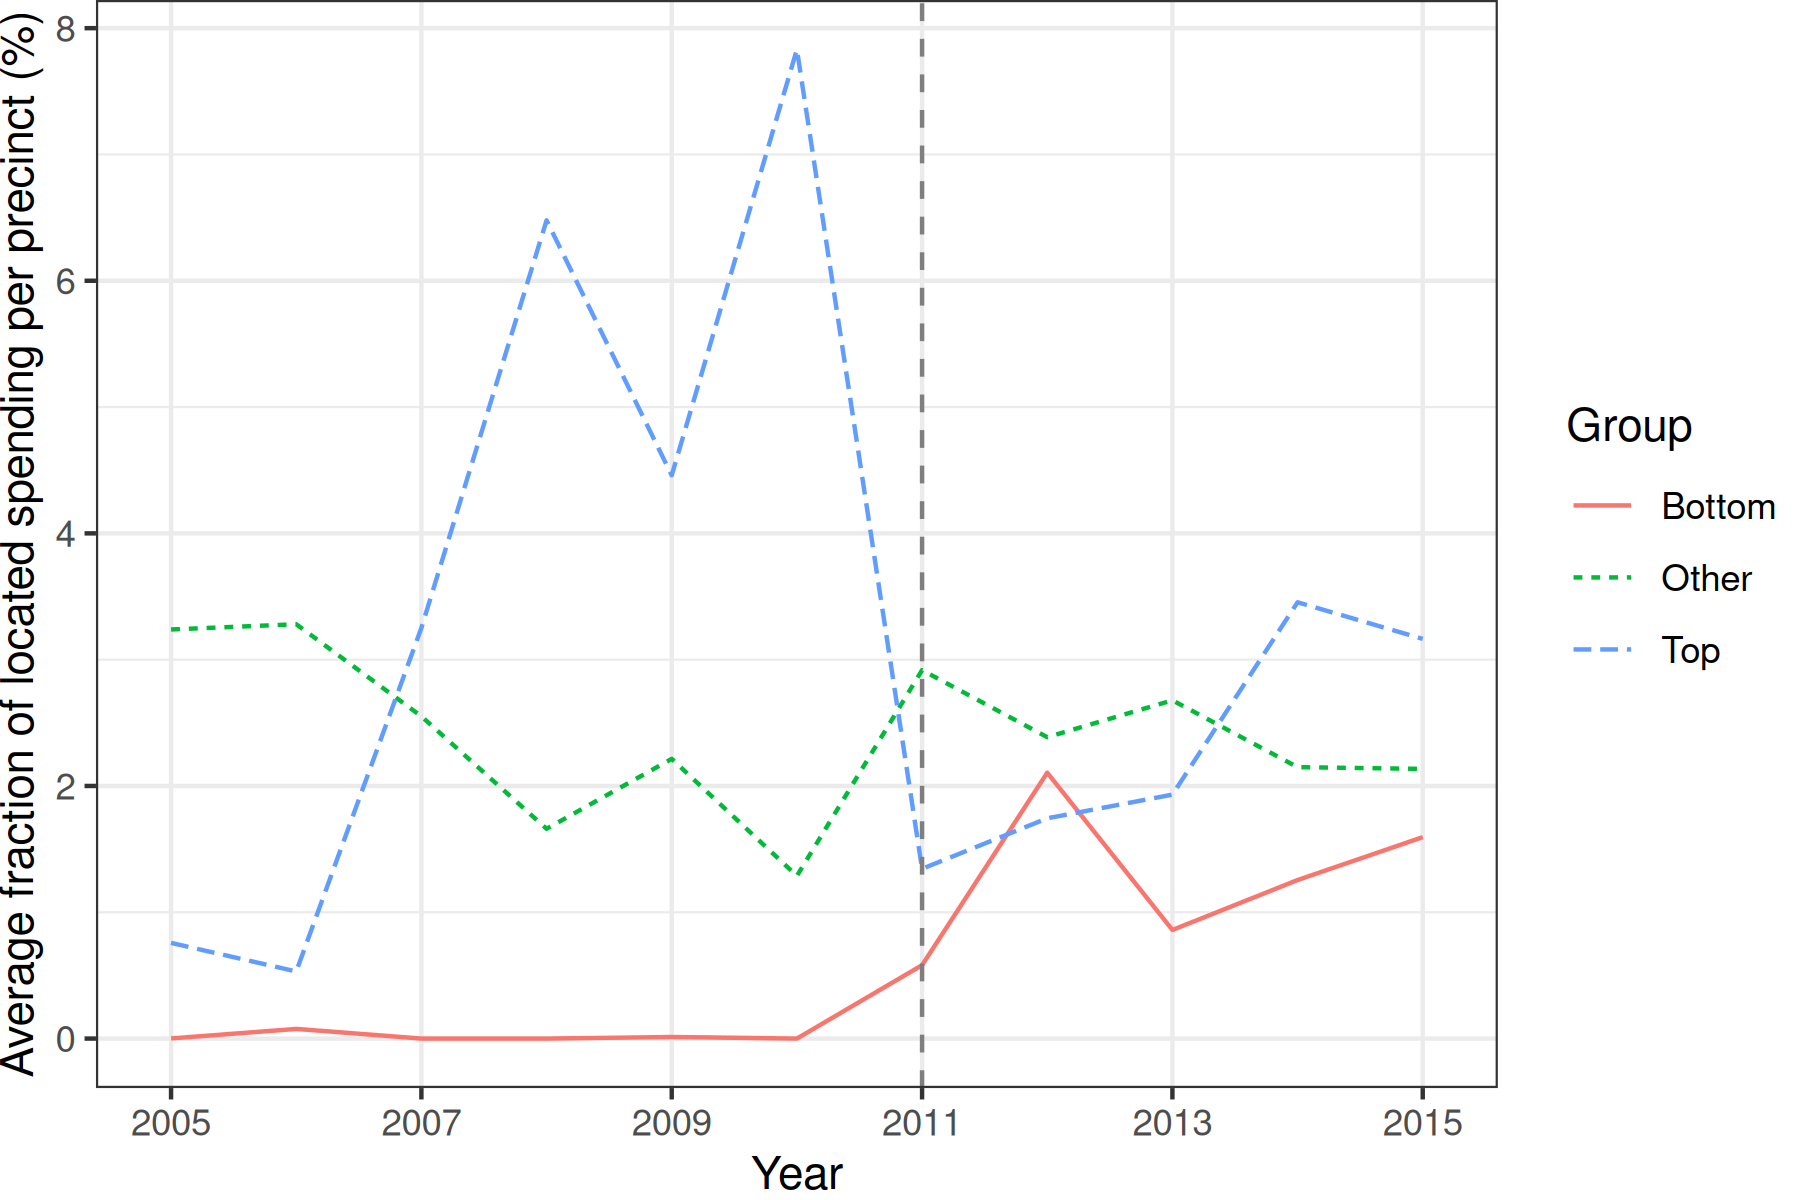
\includegraphics[width=0.65\textwidth]{input/ward_50_contribution_8_precincts_timeline.png}
    \caption{Average spending by precinct group in the 50th ward, 2005-2016}
    \label{fig:stone_spending_timeline}
\end{figure}

Figure~\ref{fig:stone_spending_maps} shows the shift geographically. 
It demonstrates a clear movement away from the south-western portion of the ward to a roughly even distribution after Stone's defeat.

\begin{figure}[H]
    \centering
    % First subfigure
    \begin{subfigure}[b]{0.45\textwidth} % [b] aligns at the bottom
    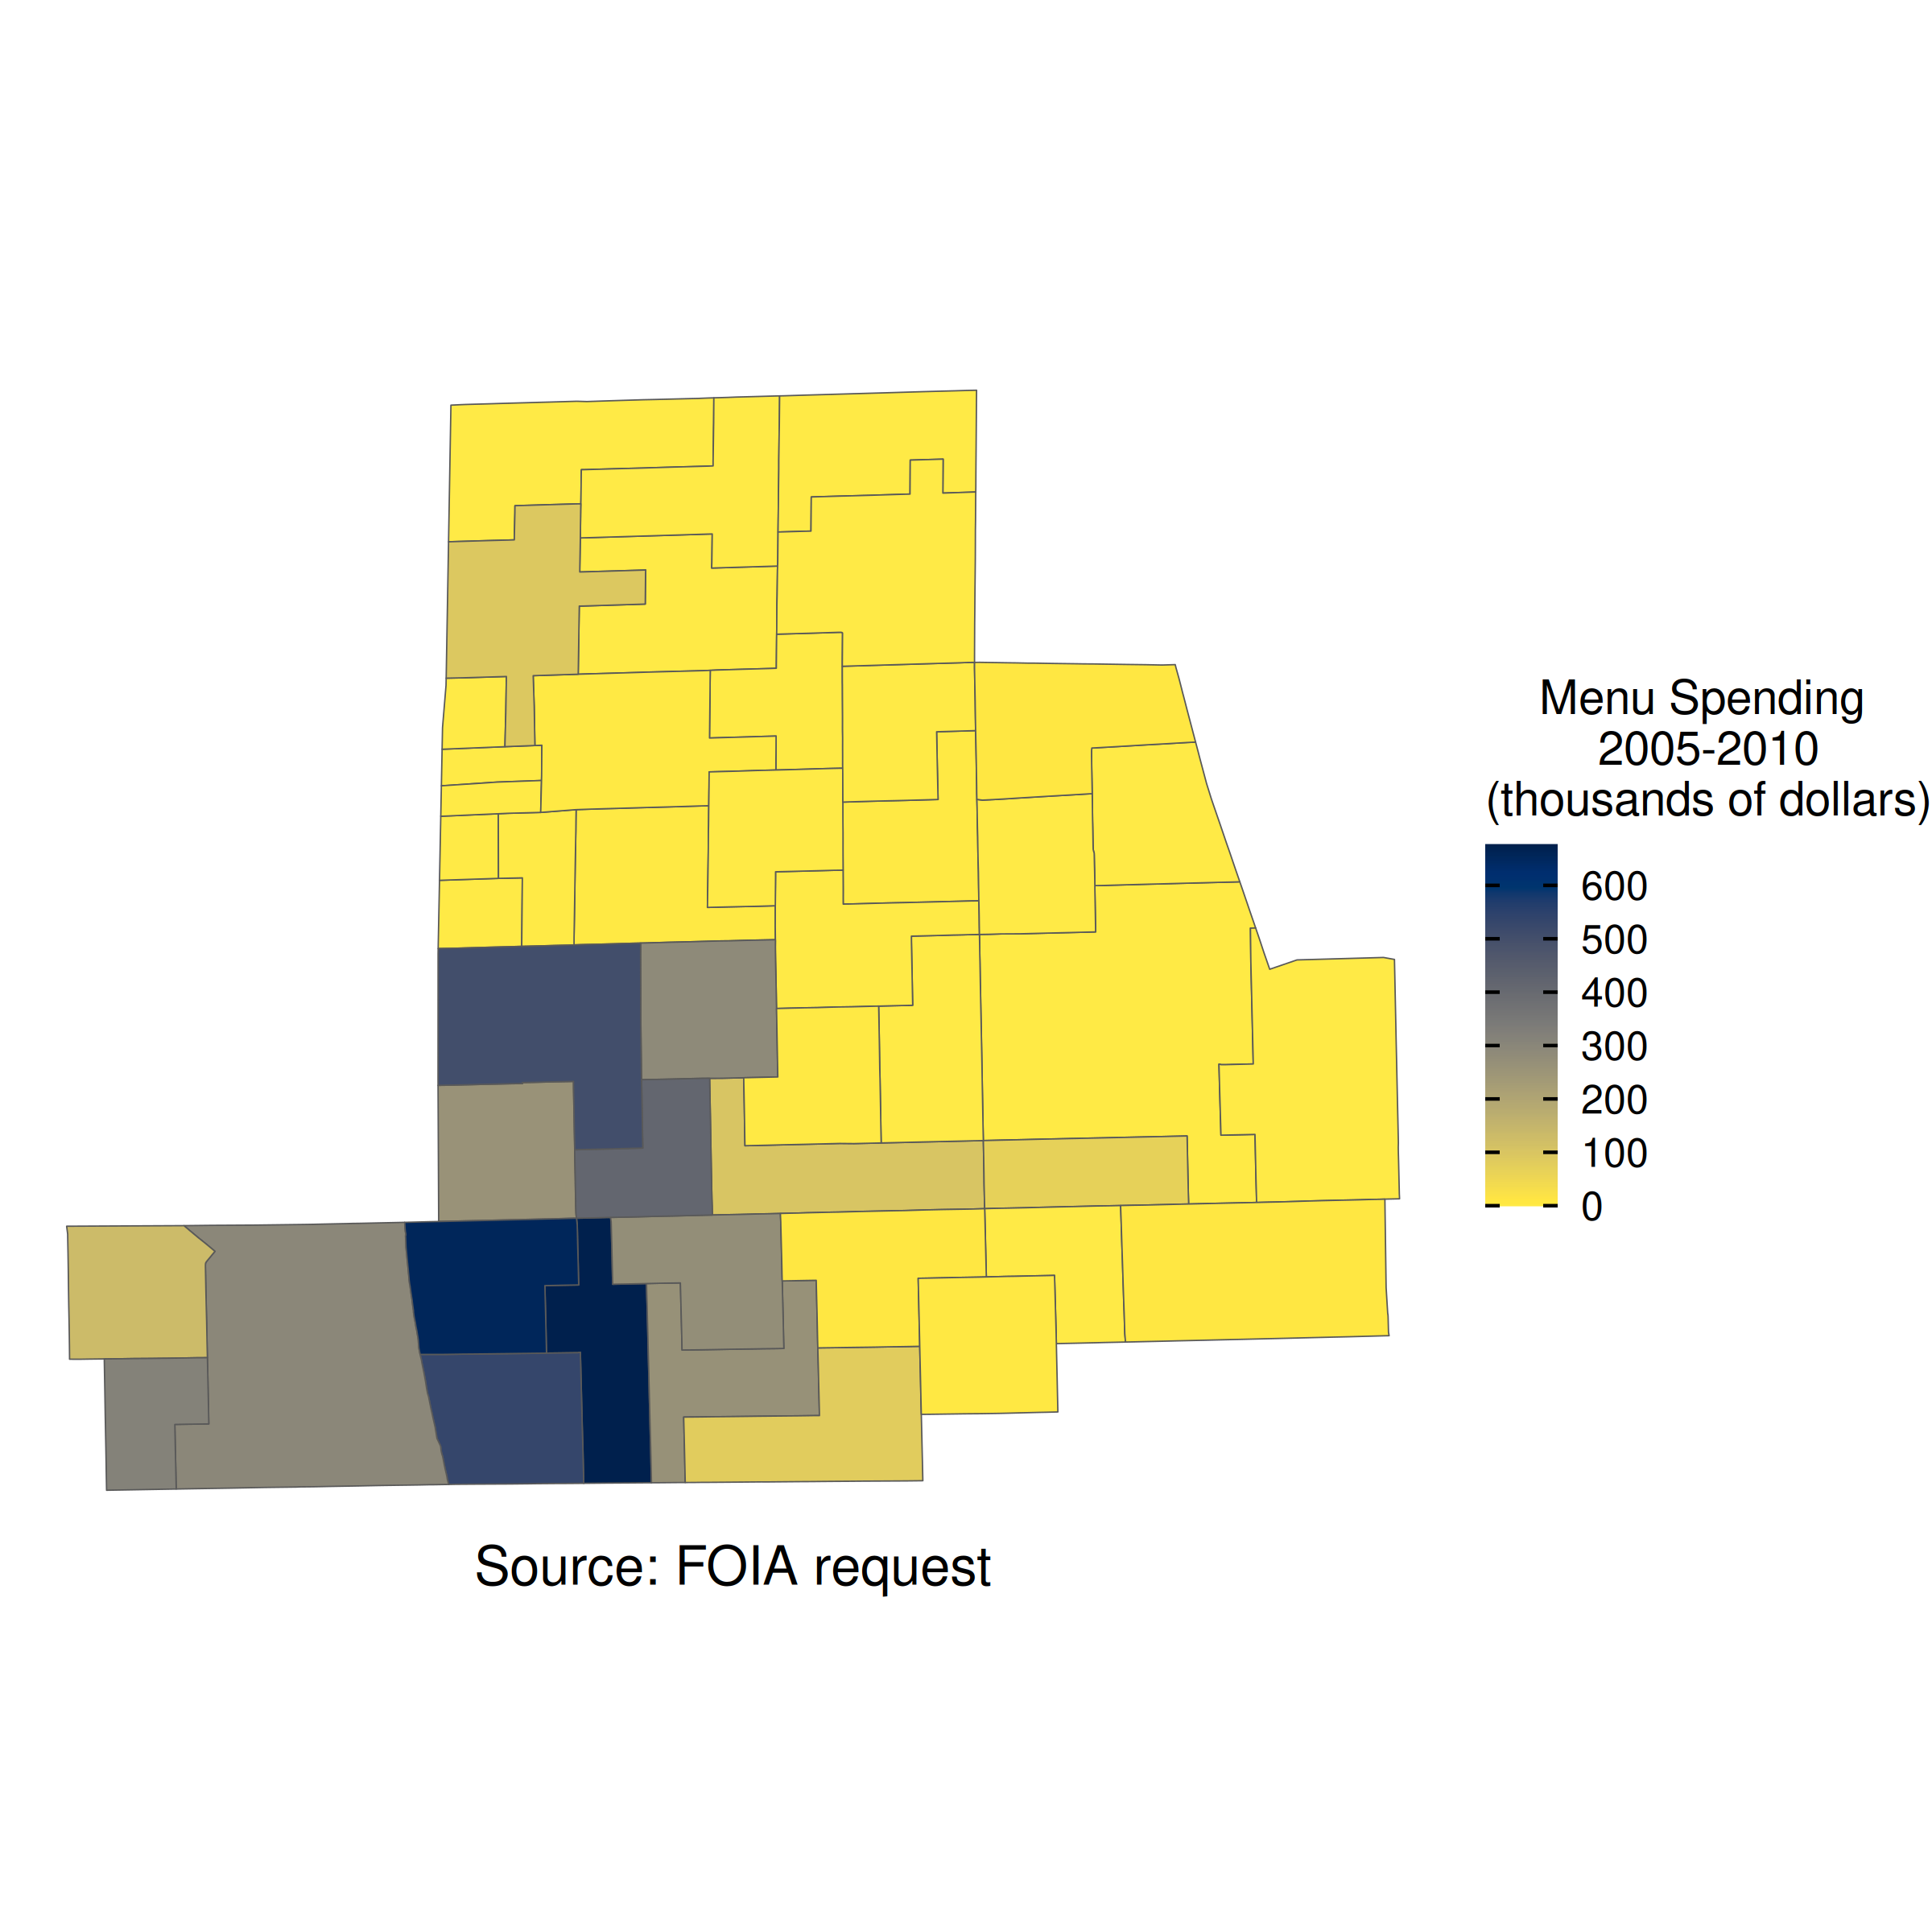
\includegraphics[width=\textwidth]{input/ward_50_menu_map_2005_2010.png}
    \caption{50th ward menu allocation, 2005-2010}
    \end{subfigure}
    \hfill % This adds some space between the two subfigures
    % Second subfigure
    \begin{subfigure}[b]{0.45\textwidth}
    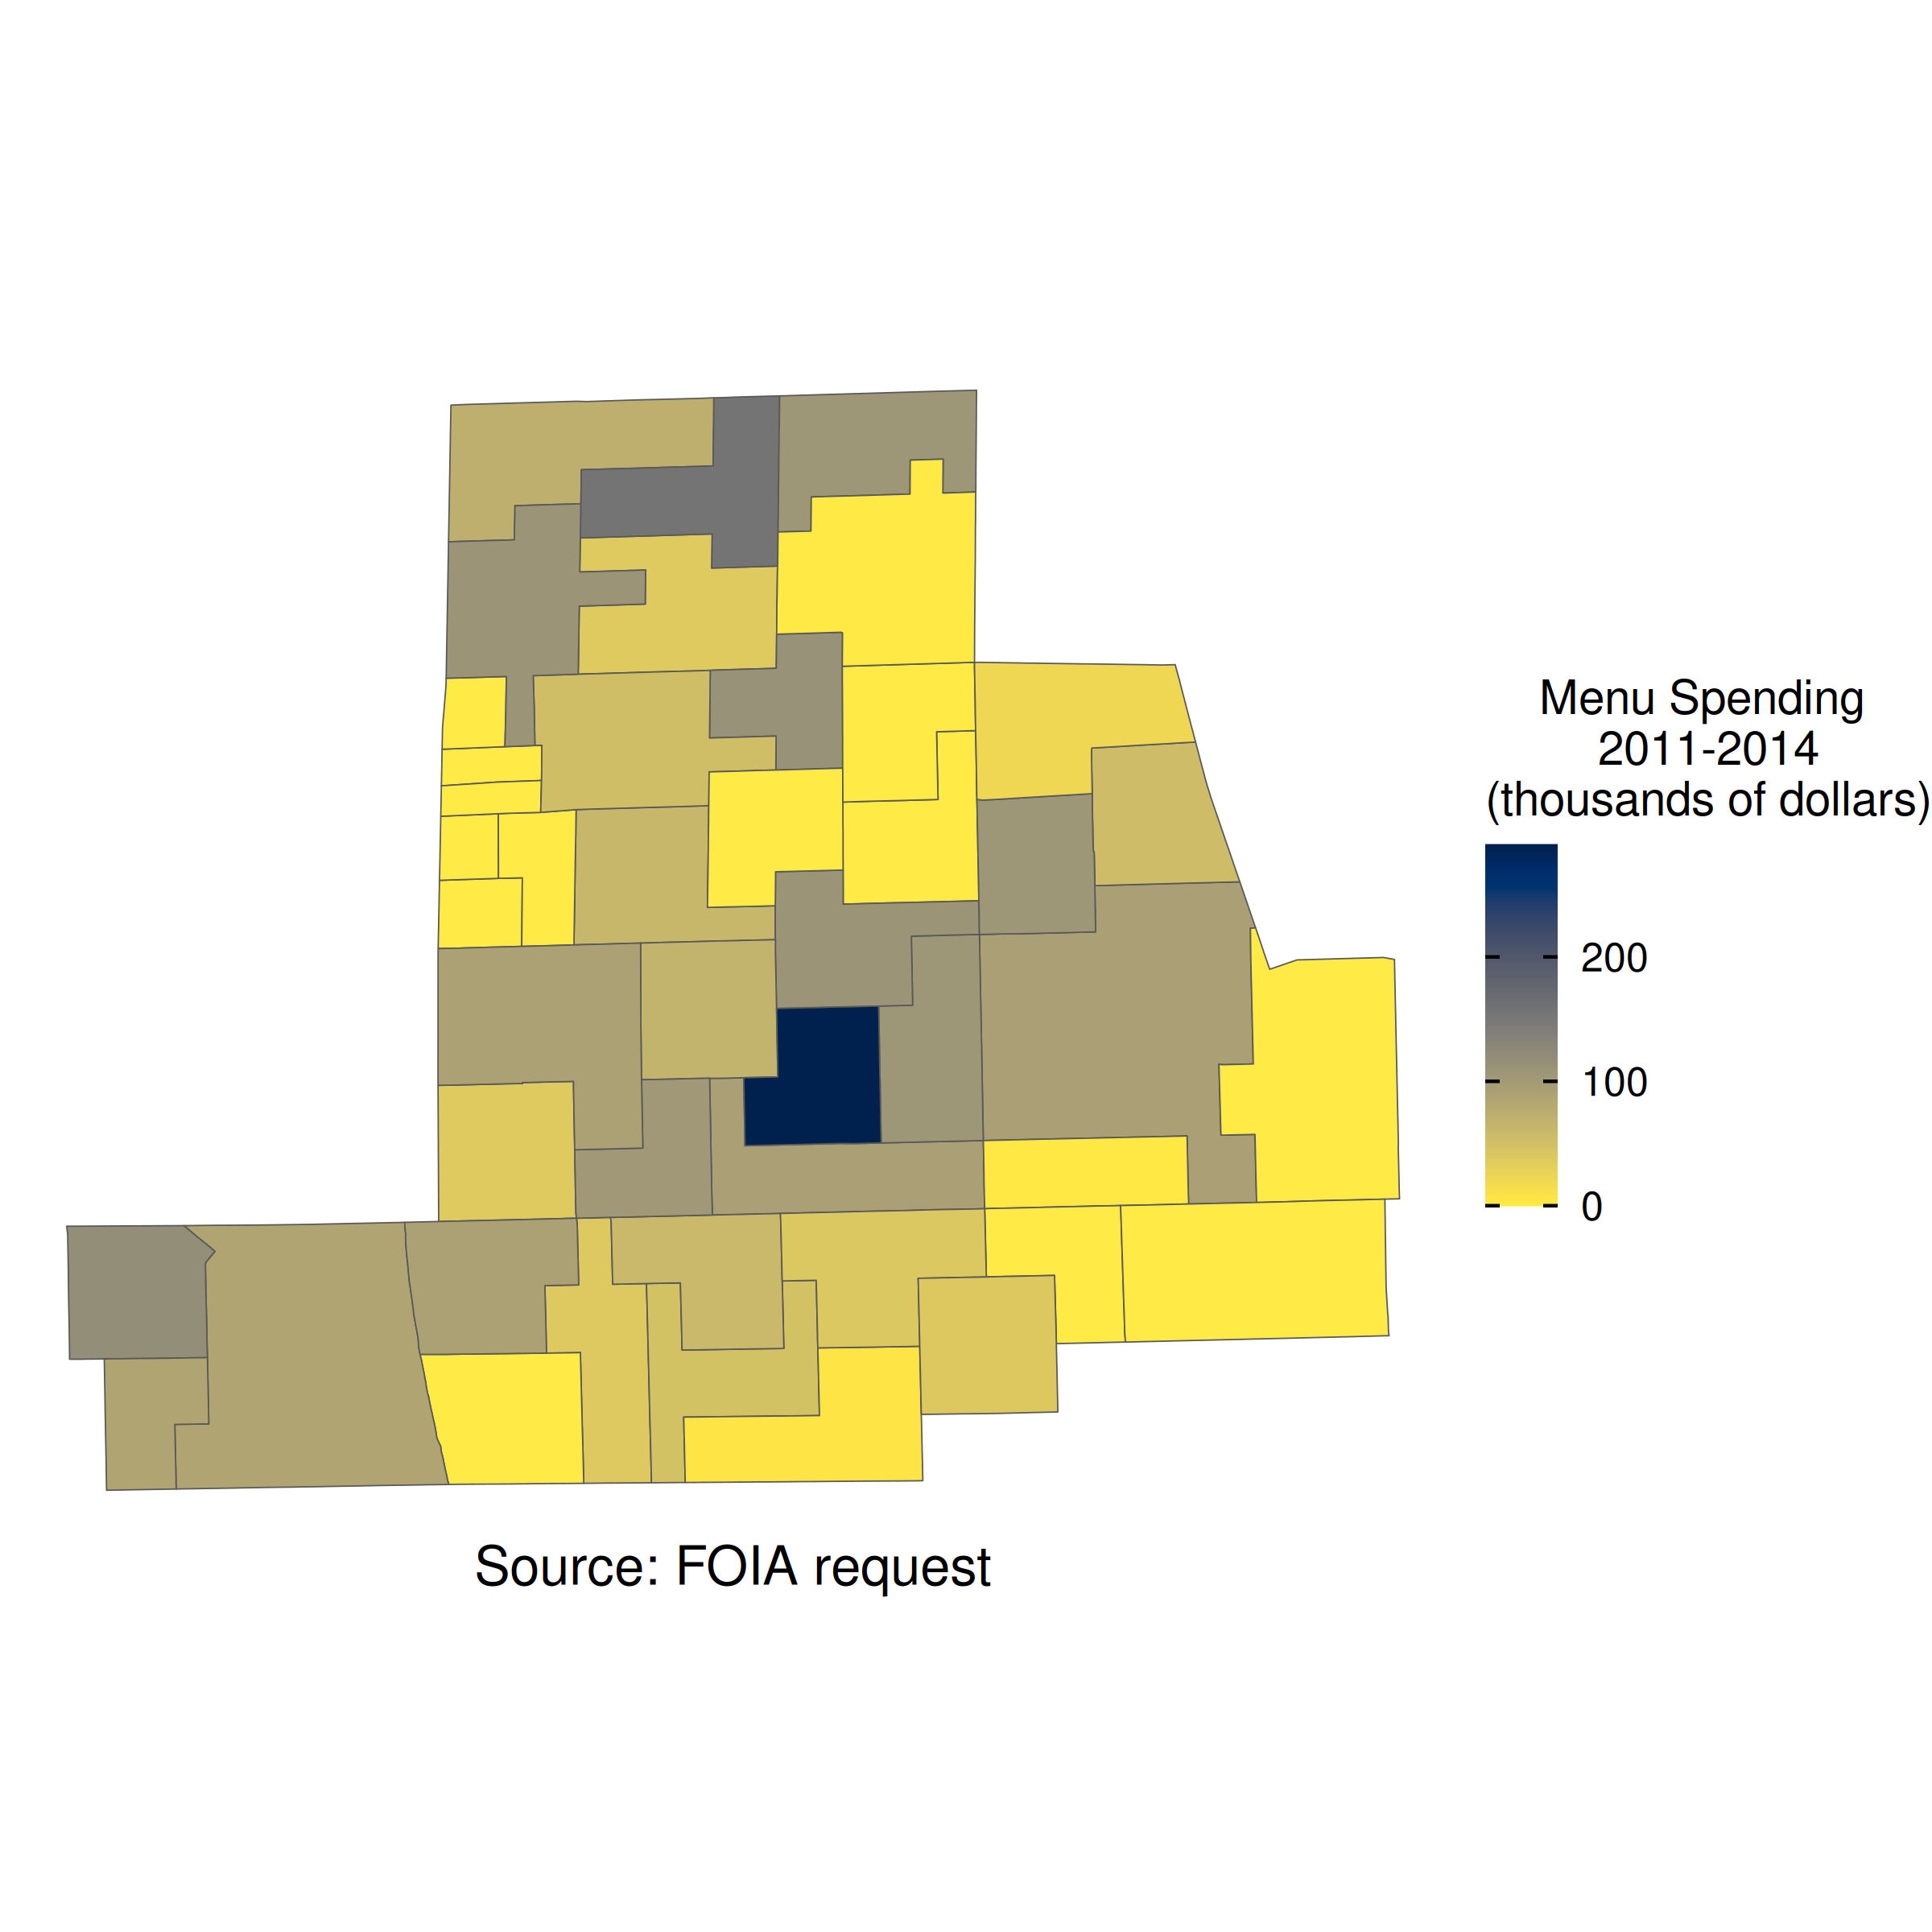
\includegraphics[width=\textwidth]{input/ward_50_menu_map_2011_2014.png}
    \caption{50th ward menu allocation, 2011-2014}
    \end{subfigure}
    \caption{50th ward menu maps before and after Stone's defeat}
    \label{fig:stone_spending_maps}
\end{figure}

